\documentclass[UTF8, a4paper]{ctexart}
\usepackage{color}
\usepackage{anyfontsize}
\usepackage{extarrows}
\usepackage{amsthm}
\usepackage{caption}
\usepackage{geometry}
\usepackage{listings}
\usepackage{graphicx}
\usepackage{subfigure}
\usepackage{mathabx}  
\usepackage[ruled,linesnumbered]{algorithm2e}
\usepackage{amsmath} 
\usepackage{amsfonts,amssymb}

\geometry{left = 2.18cm, right = 2.18cm, top = 1.54cm, bottom = 1.54cm}

\begin{document}
\definecolor{grey}{RGB}{125, 125, 125}
\definecolor{MyGreen}{RGB}{0, 125, 0}
\centerline{\textbf{\LARGE{操作系统实验报告Lab2}}}
\bigskip
\centerline{\large{成员:陈豪斌 \quad 朱浩泽 \quad 许佳培}}
\bigskip
    在这之前我们必须详细地了解uCore启动分页机制的原理是什么。
    最开始在GCC对操作系统编译的时候,会根据GNU链接脚本调用kern entry这一段汇编代码,
    并且这段代码将系统载入的地址设置在0xC01000000(即KERNBASE)处,
    因此设置REALLOC函数就很有必要了,不然一段地址可能会访问到错误的地方。
    其中,kern entry设置入口点的代码在kern/init/entry.S中,它主要是将一
    级页表的基地址,即boot\_pgdir载入寄存器cr3中(Control Register 3),
    随后将cr0的PG标志位设置上,标志分页机制已经开启。
    \par 
    在做好这些工作之后,kern\_init函数也就可以正常地执行了。
    \bigskip
    \par 
    我们主要关注物理内存管理器的初始化函数pmm\_init是如何填充页表、对pmm进行初始化的。
    \begin{enumerate}
        \item boot\_cr3 = PADDR(boot\_pgdir) :获取一级页表的基地址,注意entry.S和kernel.ld完成了将其读入的过程,因此我们可以
              轻松获取基地址。注意到在entry.S中,movl \%eax, \%cr0指令结束后,在实模式下的uCore实际上已经开启了分页机制。
              这部分会开启一种类似于页表的自映射机制。
        \item pmm\_init() :初始化pmm\_manager,我们实现了First Fit算法,因此让其指向default版本,如果想要实现别的,可以让它指向一个我们实现的manager;
        \item page\_init() :物理内存探测,检测哪些内存区域可用。这个函数比较重要,需要着重进行分析:
            {
                \begin{enumerate}
                    \item 首先这个函数会获取一个叫做e820map的结构体。
                            \par
                            e820 is shorthand for the facility by which the BIOS of x86-based computer systems reports the memory map to the operating system or boot loader.
                            \par
                            这个E820的获取,需要联系BootLoader的加载过程。关注bootasm.S文件中有关probe memory小节的描述,最重要的部分是它向
                            CPU发送了一个int 15H的中断,以及设置AX低位为E820(movl \$0xE820, \%eax),那么这个中断会让CPU返回一个关于内存区域的报告信息,即E820结构。它被存到了离内核基址8000
                            的内存处,所以根据KERNBASE + 0x8000就可以获取到内存分布的E820结构了。
                \end{enumerate}
            }
    \end{enumerate} 


\begin{enumerate}
    \item [一、] \textbf{实现First Fit算法}
    \par
    首先我们需要分析代码中是如何组织空闲内存块的。
    实际上在代码中并非单独创建某个结构体用以表示block,而是定义了一个叫做Page的结构,然后以每个block的基址Page来标识各个块,作为它们的Identifier。
    这样的话就可以支持地址的比较了,因为,我们只需要定义一个指向Page的指针即可。指针的值就是它指向的元素的地址,因此,地址的比较可以在指针的运算的基础上完成。详情可见下图:
    \begin{figure}[!htb]
        \centering
        \includegraphics[scale=0.25]{freelist.png}
        \label{fig:1}
        \caption{free\_list和空闲内存块}
    \end{figure}
    \par
    例如,假设我们想要访问block 1中的page 2,我们先要设置一个指针指向free\_list的开始位置,随后将每个list\_entry类型的指针,通过一个叫做
    le2page的函数转换为page后判断property,然后设置基址指针为它,在基址的基础上增加偏移量即可访问任意page。随后的free和alloc函数也是基于指针和指针
    与page之间的转换而实现的。如果想要将page作为遍历free\_list的指针使用,就可以直接利用它的成员变量list\_link即可。
    \par
    对各个函数的模块功能解释:
    \begin{enumerate}
        \item [1.] 有关defualt\_init函数:它初始化free\_list。这个过程很简单,它把头尾指针都指向自身即可;
        \item [2.] 有关defualt\_init\_memmap函数:在一个块被分配之后我们需要把它进行初始化。因此它遍历块中的各个page,将其状态都设置为空闲,把reference标志位清空等。
                   特别地,如果page恰好是这个块的初始页,那么我们需要将其的property设置成块的大小。 因为我们想要实现FF算法,所以,必须要根据地址进行排序,那么通过指针比较即可实现这个
                   地址排序功能。此处就须将每个初始化好的块放置到free\_list的起始部分。
        \item [3.] 有关default\_alloc\_pages函数:显然我们需要遍历free\_list这个链表来查看是否一个块满足我们所需的要求,即某个page的property(如果不为0,它代表了块的页数量)大于等于n(所需大小)。在分配完这一个内存块后,我们需要把剩余的空间(如果有的话)
                   作为一个新的内存块链入当前分配完的内存页的后面。这一步可以很轻松地使用指针完成。假设当前被分配的块的标识符是base,所需的大小为n,那么我们只需要将base + n之后的指针作为一个新块链入到base + n之后即可,与此同时我们需要将base从空闲链表上摘下,然后
                   设置base + n之后的内存块的大小为原始块大小减去n,再将其链入base + n指针之后(通过list\_add\_after实现)。
        \item [4.] 有关default\_free\_pages函数:这个函数是将一个用完的内存块链入free\_list并对碎片进行整理的函数(原函数并没有完全实现)。这个过程实际上也很简单。第一步,我们需要清空要释放的内存块的所有page;第二步,我们需要遍历free\_list链表,找到能够合并的块:有两种可能,一是某个块可以和前面的块合并,
                   二是一个块能和它后面的块合并,所以会有一个分支检测。怎么判断两个块恰好能合并呢?显然可以通过base的地址加上块大小是否和前后的块的起始地址相等进行判断。第三步,将空闲的块链入free\_list中,这一步需要保持地址有序,所以依旧需要遍历链表,找到第一个地址恰好比要插入的块小的那个块,然后调用add\_before
                   函数链入。P.S.如果先链入再合并会导致这个空闲块没法和前后块合并了。
    \end{enumerate}
    那么是否还有优化的余地呢?我们分析可见,实际上最花费时间的是遍历链表的过程,但是根据地址排序的链表想要找到第一个大小满足所需的block是无法优化的,只有一处可以优化:插入。因为插入是根据地址进行的,并非通过块大小,这意味着如果我们能够优化
    插入过程,就有希望优化部分时间复杂度。自然可以联想到使用二叉搜索树之类的树结构实现。不过可能需要保存一份free\_list的拷贝,并且单纯使用二叉搜索树可能会导致树深度过大,因此使用红黑树或者AVL树可能会是更好的解决方案。

    \item [二、] \textbf{实现寻找虚拟地址对应的页表项。}
    在实现之前,我们首先需要分析现代操作系统中是如何实现分页机制的。第一,对于每个进程而言,它都有自己的页表,这样能够实现每个应用程序都以为自己拥有全部的内存空间,而应用程序发起的虚拟地址请求将会被
    内存管理单元(Memory Management Unit)截获。第二,通过查询页表,将对应的物理地址传送回来,MMU在此过程中相当于是一个翻译器。那么,为了查询页表,我们首先需要知道页表的地址在哪里,这就需要一个叫做
    Page Directory Table的表,它能够返回每个进程发起的虚拟地址请求的对应页表地址。原理图如下图所示:
    \begin{figure}[!htb]
        \centering
        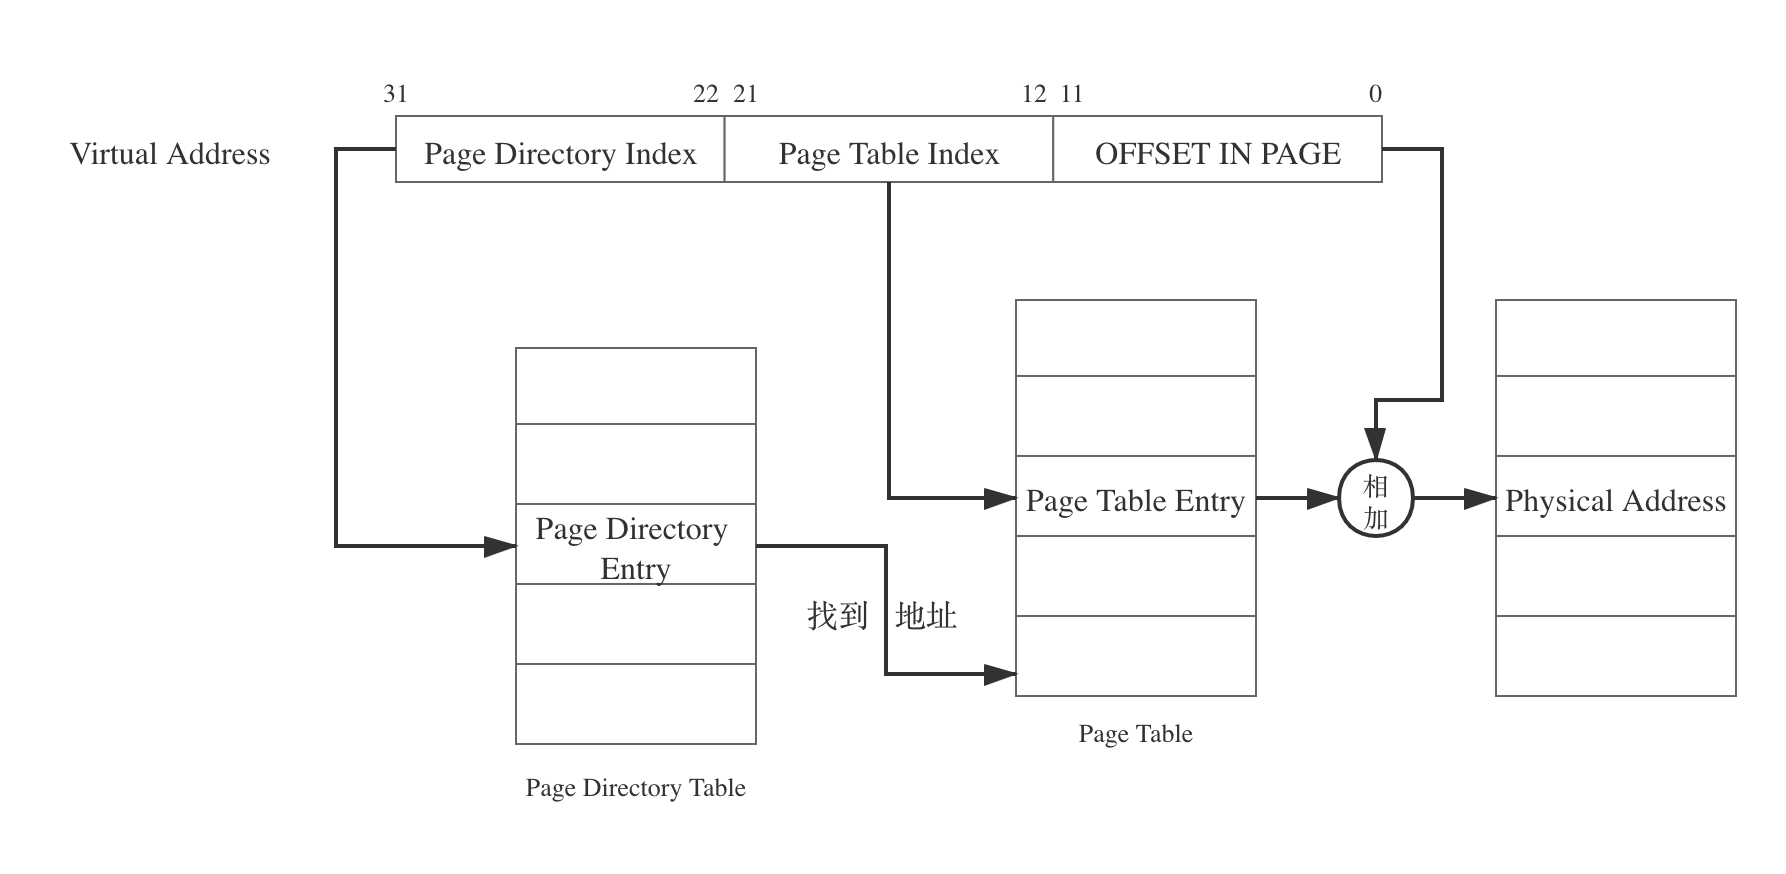
\includegraphics[scale=0.25]{paging.png}
        \label{fig:1}
        \caption{页表、页表的表和虚拟地址转换机制}
    \end{figure}
    \par
    另,若页表的表访问发生缺失,说明这个进程刚刚创建,所以我们需要为其开辟一片新的页(根据create变量来判断)。随后,我们需要将访问的页设置为referenced。
    故函数实现方式如下:
    \begin{enumerate}
        \item [1.] 根据虚拟地址的高位和页表的表的基址,找到对应于这个虚拟地址的页表的地址。如果不存在,就需要分配一片新的内存页给页表的表,并对内容初始化为0,状态位重设;
        \item [2.] 接下来通过PTE\_ADDR函数,获取这个Page Directory Entry(即页表的表中的某一项)指向的页表地址;
        \item [3.] 根据第二步找到的页表地址,加上虚拟地址中间一部分对应的页表内的偏移,形成最终的页表项返回。
    \end{enumerate}
    \end{enumerate}
\end{document}